% Figure -- generation-vs-representation envelope (FID + designability). \input{} from Ch6.
\begin{figure}[tbp]
\centering
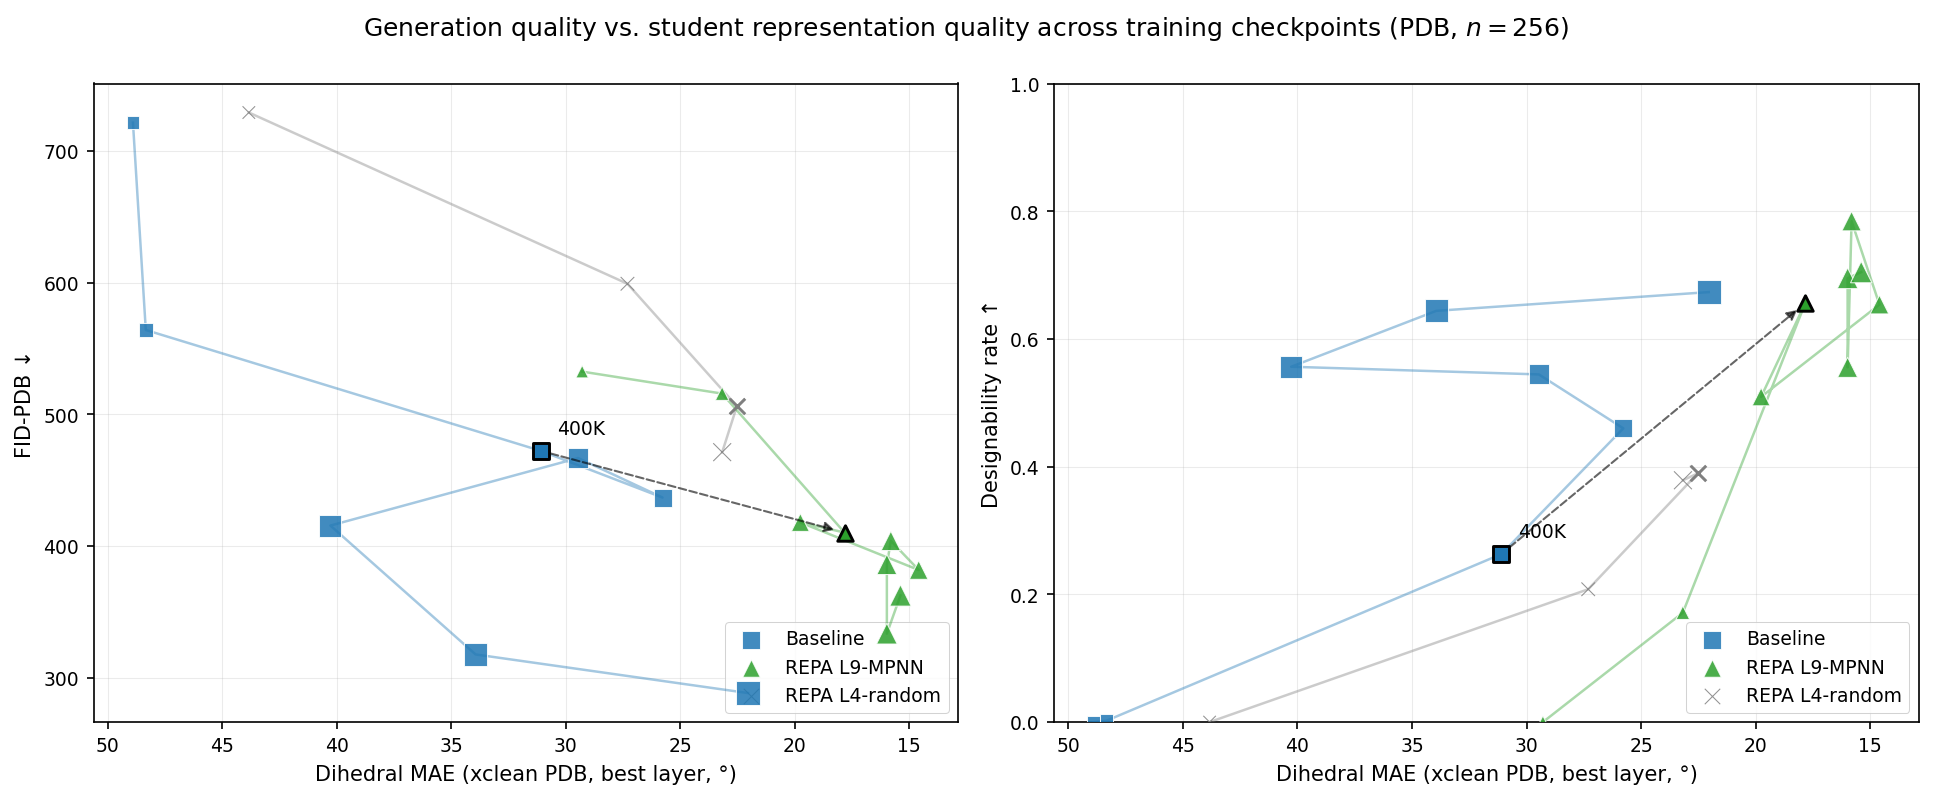
\includegraphics[width=\textwidth]{figures/fig04_fid_des_gen_vs_rep.png}
\caption{\textbf{Better student geometry buys better generation at equal compute --- direct evidence REPA relieves the representation bottleneck.} Generation quality against representation quality, $n=256$ PDB, one marker per checkpoint. The $x$-axis is student dihedral MAE (better to the right). \emph{Left:} FID-PDB (lower is better); \emph{right:} designability (higher is better). Baseline (blue squares), REPA L9-MPNN (green triangles), and the random control (grey $\times$) lie on a common band where better dihedral geometry accompanies better generation on both metrics. The dashed arrow connects baseline and L9-MPNN at matched training compute ($\approx 400$K steps), showing REPA delivering better generation quality for the same budget.}
\label{fig:proteina-genrep}
\end{figure}
